\section{Experimentación}

\subsection{Descripción de la Experimentación}

En esta sección se cubre la parte experimental del proyecto. Todo el desarrollo ha sido realizado utilizando Knime, una herramienta para el análisis de datos ampliamente utilizada en este sector. El objetivo principal es ofrecer una comparación entre las diferentes métricas vistas en secciones anteriores, poniendo especial énfasis en la comparación de estas con el nuevo método grafico curva-A.

\bigbreak

Para la experimentación vamos a partir de una selección de seis ficheros de datos, todos los ficheros utilizados en la experimentación han sido obtenidos de la web del SBCB \url{https://sbcb.inf.ufrgs.br/cumida}, en general los conjuntos de datos forman parte de un repositorio de datos relacionado con diversos tipos de cáncer, estos conjuntos de datos cubren un amplio rango de casuísticas y suponen una excelente elección para entrenar modelos tanto de clasificación binaria como modelos de clasificación multi etiqueta.

\bigbreak

El escenario de pruebas que se ha definido no se realiza ningún tipo de preprocesado al conjunto de datos de entrada, únicamente se aplica una normalización, ya que supone una mejora en el rendimiento de los modelos basados en el teorema de Bayes. Para los diferentes conjuntos de datos, se va a aplicar un predictor basado en el teorema de Bayes. Para la validación aplicamos validación cruzada con 10 iteraciones, el uso de este tipo de validación está muy extendido en proyectos de análisis de datos, ya que ofrece en general grandes resultados. Para cada fichero presentaremos los resultados obtenidos fruto de aplicar las métricas vistas anteriormente al conjunto de datos correspondiente. Posteriormente se exponen las conclusiones.


\clearpage

\subsection{Resultados de la Experimentación}


%%%%%%%%%%%%%%%%%%%%%%%%%%%%%%%%%%%%%%%%%%%%%%%%%%%%%%% RESULTADO
\subsubsection{Fichero brain\_gse15824.csv}

\begin{table}[htp]
    \small
    \centering
    \begin{tabularx}{\columnwidth}{Y Y}
        ACC       & AUAC    \\\hline
        $0.757$   & $0.764$ \\\hline
    \end{tabularx}
    \caption{Resultados globales para el fichero brain\_gse15824.csv.}
    \label{tab:10}
\end{table}

\begin{table}[htp]
    \small
    \centering
    \begin{tabularx}{\columnwidth}{l c c c c}
                &  Astrocytoma  & Glioblastoma & Oligodendrioglioma   & Glioblastoma-cell-line   \\\hline
        TPR     &  $0.500$      & $1.000$      & $0.286$              & $1.000$                  \\\hline
        TNR     &  $0.966$      & $0.720$      & $0.967$              & $1.000$                  \\\hline
        PPV     &  $0.800$      & $0.632$      & $0.667$              & $1.000$                  \\\hline
        NPV     &  $0.875$      & $1.000$      & $0.853$              & $1.000$                  \\\hline
        LR+     &  $14.500$     & $3.571$      & $8.571$              & -                        \\\hline
        LR-     &  $0.518$      & $0.000$      & $0.739$              & $0.000$                  \\\hline
        DOR     &  $28.000$     & -            & $11.600$             & -                        \\\hline
        YI      &  $0.466$      & $0.720$      & $0.252$              & $1.000$                  \\\hline
        MCC     &  $0.561$      & $0.674$      & $0.362$              & $1.000$                  \\\hline
        DP      &  $0.798$      & -            & $0.587$              & -                        \\\hline
        $F_{1}$ &  $0.615$      & $0.774$      & $0.400$              & $1.000$                  \\\hline
        MK      &  $0.675$      & $0.632$      & $0.520$              & $1.000$                  \\\hline
        BCR     &  $0.733$      & $0.860$      & $0.626$              & $1.000$                  \\\hline
        GM      &  $0.695$      & $0.849$      & $0.526$              & $1.000$                  \\\hline
        OP      &  $0.547$      & $0.648$      & $0.294$              & $1.000$                  \\\hline
        Jaccard &  $0.444$      & $0.632$      & $0.250$              & $1.000$                  \\\hline

    \end{tabularx}
    \caption{Resultados agrupados por clase para el fichero brain\_gse15824.csv.}
    \label{tab:11}
\end{table}

\bigbreak

\begin{figure}[htp]
    \centering
     \subfloat[Curva ROC]{
       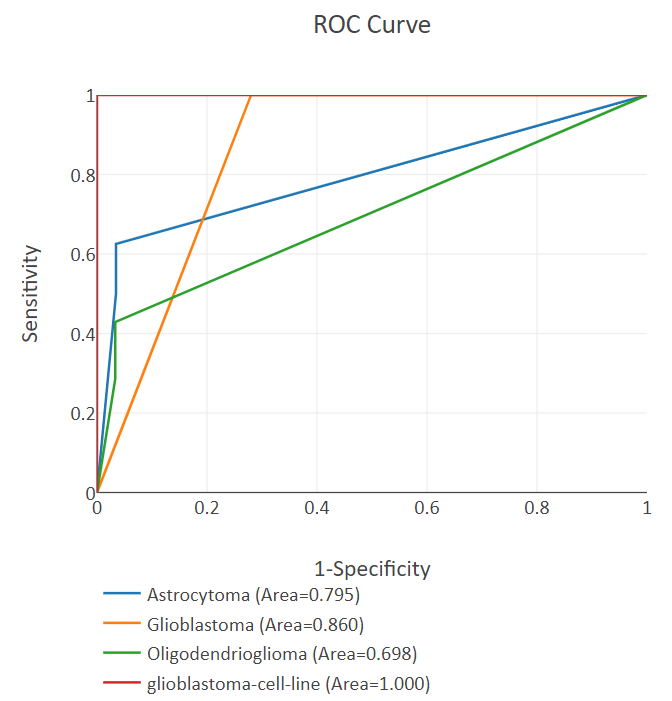
\includegraphics[width=0.4\textwidth]{brain_gse15824_ROC.PNG}}
     \subfloat[Curva A]{
       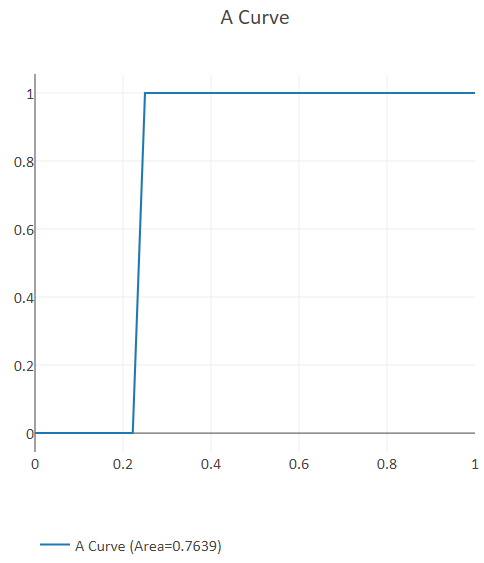
\includegraphics[width=0.4\textwidth]{brain_gse15824_A_CURVE.PNG}}
    \caption{Curvas obtenidas para el fichero brain\_gse15824.csv.}
    \label{fig:10}
\end{figure}

\bigbreak

El fichero de datos brain\_gse15824.csv presenta cuatro clases, los nombres de las clases son Astrocytoma, Glioblastoma, Oligodendrioglioma y Glioblastoma-cell-line. En esta sección se ofrece un análisis e interpretación de los resultados obtenidos al aplicar los métodos de evaluación vistos en secciones anteriores. El análisis e interpretación se realiza de forma independiente para las diferentes clases.

\bigbreak

La exactitud es de $0.757$ unidades, es decir, hay un $75.7$\% de probablidad de acierto en la predicción que realiza el modelo. El área bajo la curva-A es de $0.764$ unidades, un valor notablemente alto. La diferencia entre el área bajo la curva-A y la exactitud es de $0.007$ unidades. 

\bigbreak

La clase Astrocytoma presenta un indicador de sensibilidad bajo, un resultado de $0.5$ indica que tan solo la mitad de los registros de está clase se prediccen de forma correcta. La especificidad es de $0.966$ unidades, esto implica que para intancias en las que la clase es diferente a Astrocytoma, la predicción se hace correctamente el 96.6\% de las veces. El indicador de precisión es de $0.8$ unidades, las instnacias que se predicen de clase Astrocytoma tienen una tasa de acierto del $80$\%. La precisión inversa indica que la predicción es correcta para el 80\% de las instancias que se predicen de una clase diferente a Astrocytoma. El resultado para la precisión inversa es de $0.85$ unidades, la tasa de aciertos en la prediccón de clases diferentes a Astrocytoma es notablemente buena. La razón de verosimilitud positiva presenta un fuerte aumento de la probabilidad de acierto que tiene un registro que se predice de clase Astrocytoma, en concreto supone más de un 45\% de mejora (Tabla \ref{tab:2}). La razón de verosimilitud negativa obtiene un resultado de $0.518$ puntos, esto implica una leve disminución en la probabilidad de que un registro sea de clase Astrocytoma cuando se precdice de una clase diferente, la disminución que presenta es de entorno al 15\% (Tabla \ref{tab:2}). El DOR ofrece un indicador conjunto de las razones de verosimilitud, en general indica una buena capacidad discriminatoria para la clase Astrocytoma. El indice de Youden tiene un valor de $0.46$, un valor poximo a $0.5$ indica una capacidad discriminatoria aceptable para la clase Astrocytoma. El resultado para el coeficiente de correlación de Matthews es de $0.561$ unidades, un valor que indica una fuerte correlación entre clase y predicción (Tabla \ref{tab:3}). El poder disciminante de $0.798$ implica una capacidad discriminatoria postiva para la clase Astrocytoma. El valor de la medida-F implica una tasa aceptable de acierto para instancias en las que la clase o la predicción es Astrocytoma, en este caso la baja sensibilidad obtenida penaliza el resultado obtenido. El markedness es un indicador que agurpa los métodos que miden la exactitud en la predicción, un resultado de $0.675$ implica una notable tasa de acierto. La media geometica y la exactitud balanceada ofrecen un indicador de la tasa de acietos conjunta para instancias de clase Astrocytoma e instancias que no son de clase Astrocytoma, en ambos casos el indicador es notablemente alto. El resultado para la precisión de optimización es de $0.547$ unidades, un valor bajo que se ha visto afectado por la gran diferencia que existe entre sensibilidad y especificidad. El resultado que se obtiene al aplicar Jaccard es de $0.444$ unidades, esto indica un grado de similitud bajo entre clase y predicción.

\bigbreak

La sensibilidad para la clase Glioblastoma es de una unidad, esto implica que todas las instancias de esta clase se clasifican de forma correcta. El indicador de especificidad indica una notable tasa de acierto a la hora de determinar que instancias no pertenecen a la clase Glioblastoma. La precisión de $0.63$ unidades implica una buena tasa de acierto sobre las intancias que se predicen de clase Glioblastoma. La precisión inversa obtiene un resultado de una unidad, la predicción es correcta para todas las instancias que se predicen de una clase diferente a Glioblastoma. La razón de verosimilitud positiva indica un leve aumento (Tabla \ref{tab:2}) en la probabilidad de que una instancia pertenezca a la clase Glioblastoma cuando se predice de esta clase. El indice de Youden indica una capacidad discriminatoria notable para la clase Glioblastoma. El resultado obtenido por el coeficiente de correlación de Matthews es de $0.674$, este valor implica una alta correlación (Tabla \ref{tab:3}) entre la predicción y la clase Glioblastoma. La medida-F indica una tasa notable de acierto en la predicción de la clase. La media geometica y la exactitud balanceada ofrecen indicadores que reflejan una tasa de aciertos notable, ambos métodos agrupan sensibilidad y especificidad. La precisión de optimización indica una buena tasa de acierto para la clase Glioblastoma. El método de Jaccard indica un grado de similitud medio entre la predicción y la clase Glioblastoma.

\bigbreak

d

\bigbreak

La clase Glioblastoma-cell-line muuestra un comportamiento ideal, el modelo es capaz de discriminar entre esta clase y el resto de forma perfecta.

\bigbreak

Los resultados obtenidos para el fichero brain\_gse15824.csv han sido positivos, en general las tasas de acierto han sido notables. Los métodos que se aplicado ayudan a reconocer algunos puntos de mejora, en este caso, la clase Oligodendrioglioma es la que obtiene peores indicadores, el modelo puede mejorarse ajustando la predicción sobre esta clase.

\clearpage

%%%%%%%%%%%%%%%%%%%%%%%%%%%%%%%%%%%%%%%%%%%%%%%%%%%%%%% RESULTADO

\subsubsection{Fichero breast\_gse45827.csv}

\begin{table}[htp]
    \small
    \centering
    \begin{tabularx}{\columnwidth}{Y Y}
        ACC       & AUAC    \\\hline
        $0.914$   & $0.917$ \\\hline
    \end{tabularx}
    \caption{Resultados globales para el fichero breast\_gse45827.csv.}
    \label{tab:12}
\end{table}

\begin{table}[htp]
    \small
    \centering
    \begin{tabularx}{\columnwidth}{l Y Y Y Y Y Y}
                &  Her          & Basal     & Cell\_line & Luminal\_a & Luminal\_b & Normal    \\\hline
        TPR     &  $0.900$      & $0.927$   & $1.000$    & $0.862$    & $0.933$    & $0.857$   \\\hline
        TNR     &  $0.967$      & $0.982$   & $1.000$    & $0.984$    & $0.959$    & $1.000$   \\\hline
        PPV     &  $0.871$      & $0.950$   & $1.000$    & $0.926$    & $0.848$    & $1.000$   \\\hline
        NPV     &  $0.975$      & $0.973$   & $1.000$    & $0.968$    & $0.983$    & $0.993$   \\\hline
        LR+     &  $27.225$     & $50.976$  & -          & $52.586$   & $22.587$   & -         \\\hline
        LR-     &  $0.103$      & $0.075$   & $0.000$    & $0.140$    & $0.070$    & $0.143$   \\\hline
        DOR     &  $263.250$    & $684.000$ & -          & $375.000$  & $324.800$  & -         \\\hline
        YI      &  $0.867$      & $0.909$   & $1.000$    & $0.846$    & $0.892$    & $0.857$   \\\hline
        MCC     &  $0.856$      & $0.916$   & $1.000$    & $0.869$    & $0.861$    & $0.923$   \\\hline
        DP      &  $1.334$      & $1.563$   & -          & $1.419$    & $1.385$    & -         \\\hline
        $F_{1}$ &  $0.885$      & $0.938$   & $1.000$    & $0.893$    & $0.889$    & $0.923$   \\\hline
        MK      &  $0.846$      & $0.923$   & $1.000$    & $0.894$    & $0.832$    & $0.993$   \\\hline
        BCR     &  $0.933$      & $0.954$   & $1.000$    & $0.923$    & $0.946$    & $0.929$   \\\hline
        GM      &  $0.933$      & $0.954$   & $1.000$    & $0.921$    & $0.946$    & $0.926$   \\\hline
        OP      &  $0.918$      & $0.938$   & $1.000$    & $0.894$    & $0.940$    & $0.916$   \\\hline
        Jaccard &  $0.794$      & $0.884$   & $1.000$    & $0.806$    & $0.800$    & $0.857$   \\\hline
    \end{tabularx}
    \caption{Resultados agrupados por clase para el fichero breast\_gse45827.csv.}
    \label{tab:13}
\end{table}

\clearpage

\begin{figure}[htp]
    \centering
     \subfloat[Curva ROC]{
       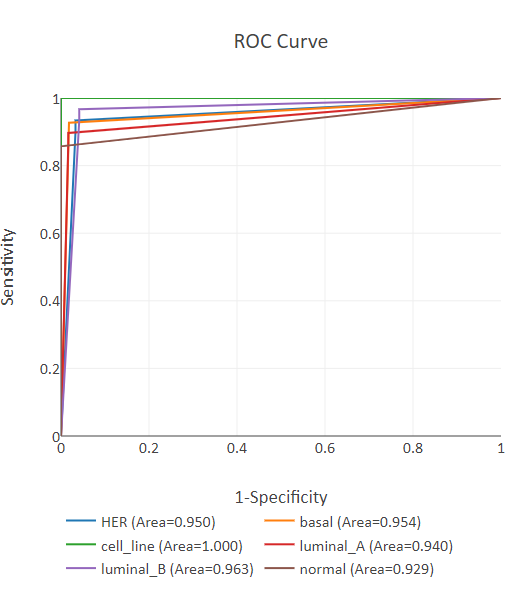
\includegraphics[width=0.4\textwidth]{breast_gse45827_ROC.PNG}}
     \subfloat[Curva A]{
       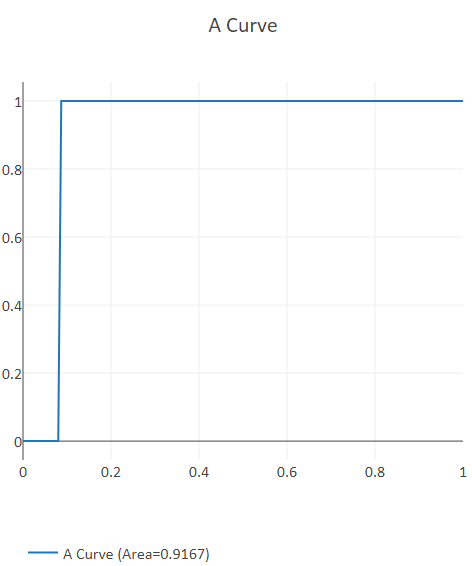
\includegraphics[width=0.4\textwidth]{breast_gse45827_A_CURVE.PNG}}
    \caption{Curvas obtenidas para el fichero breast\_gse45827.csv.}
    \label{fig:11}
\end{figure}

\bigbreak

\lipsum[1]

\clearpage

%%%%%%%%%%%%%%%%%%%%%%%%%%%%%%%%%%%%%%%%%%%%%%%%%%%%%%% RESULTADO

\subsubsection{Fichero colorectal\_gse21510.csv}

\begin{table}[htp]
    \small
    \centering
    \begin{tabularx}{\columnwidth}{Y Y}
        ACC       & AUAC    \\\hline
        $0.980$   & $0.983$ \\\hline
    \end{tabularx}
    \caption{Resultados globales para el fichero colorectal\_gse21510.csv.}
    \label{tab:14}
\end{table}

\begin{table}[htp]
    \small
    \centering
    \begin{tabularx}{\columnwidth}{l Y Y Y}
                &  Normal\_homogenized  & Tumoral\_lcm  & Tumoral\_homogenized  \\\hline
        TPR     &  $0.920$              & $1.000$       & $0.944$               \\\hline
        TNR     &  $1.000$              & $0.930$       & $1.000$               \\\hline
        PPV     &  $1.000$              & $0.972$       & $1.000$               \\\hline
        NPV     &  $0.984$              & $1.000$       & $0.992$               \\\hline
        LR+     &  -                    & $14.333$      & -                     \\\hline
        LR-     &  $0.080$              & $0.000$       & $0.056$               \\\hline
        DOR     &  -                    & -             & -                     \\\hline
        YI      &  $0.920$              & $0.930$       & $0.944$               \\\hline
        MCC     &  $0.951$              & $0.951$       & $0.968$               \\\hline
        DP      &  -                    & -             & -                     \\\hline
        $F_{1}$ &  $0.958$              & $0.986$       & $0.971$               \\\hline
        MK      &  $0.984$              & $0.972$       & $0.992$               \\\hline
        BCR     &  $0.960$              & $0.965$       & $0.972$               \\\hline
        GM      &  $0.959$              & $0.964$       & $0.972$               \\\hline
        OP      &  $0.945$              & $0.943$       & $0.965$               \\\hline
        Jaccard &  $0.920$              & $0.972$       & $0.944$               \\\hline
    \end{tabularx}
    \caption{Resultados agrupados por clase para el fichero colorectal\_gse21510.csv.}
    \label{tab:15}
\end{table}

\clearpage

\begin{figure}[htp]
    \centering
     \subfloat[Curva ROC]{
       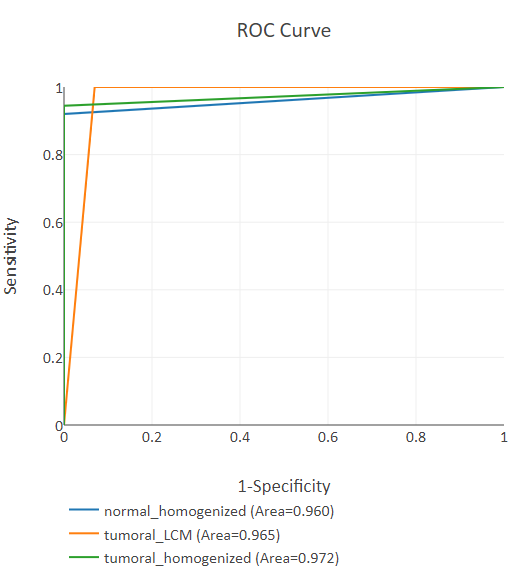
\includegraphics[width=0.4\textwidth]{colorectal_gse21510_ROC.PNG}}
     \subfloat[Curva A]{
       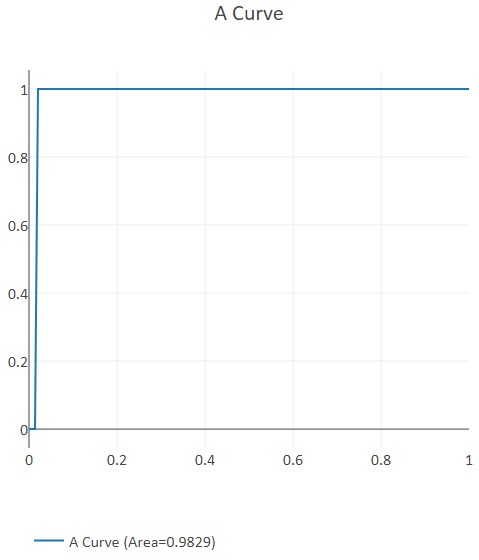
\includegraphics[width=0.4\textwidth]{colorectal_gse21510_A_CURVE.PNG}}
    \caption{Curvas obtenidas para el fichero colorectal\_gse21510.csv.}
    \label{fig:12}
\end{figure}

\bigbreak

\lipsum[1]

\clearpage


%%%%%%%%%%%%%%%%%%%%%%%%%%%%%%%%%%%%%%%%%%%%%%%%%%%%%%% RESULTADO

\subsubsection{Fichero breast\_gse42568.csv}

\begin{table}[htp]
    \small
    \centering
    \begin{tabularx}{\columnwidth}{Y Y}
        ACC       & AUAC    \\\hline
        $0.991$   & $0.996$ \\\hline
    \end{tabularx}
    \caption{Resultados globales para el fichero breast\_gse42568.csv.}
    \label{tab:16}
\end{table}

\begin{table}[htp]
    \small
    \centering
    \begin{tabularx}{\columnwidth}{l Y Y}
                &  Normal               & Tumoral       \\\hline
        TPR     &  $0.933$              & $1.000$       \\\hline
        TNR     &  $1.000$              & $0.933$       \\\hline
        PPV     &  $1.000$              & $0.990$       \\\hline
        NPV     &  $0.990$              & $1.000$       \\\hline
        LR+     &  -                    & $15.000$      \\\hline
        LR-     &  $0.067$              & $0.000$       \\\hline
        DOR     &  -                    & -             \\\hline
        YI      &  $0.933$              & $0.933$       \\\hline
        MCC     &  $0.961$              & $0.961$       \\\hline
        DP      &  -                    & -             \\\hline
        $F_{1}$ &  $0.966$              & $0.995$       \\\hline
        MK      &  $0.990$              & $0.990$       \\\hline
        BCR     &  $0.967$              & $0.967$       \\\hline
        GM      &  $0.966$              & $0.966$       \\\hline
        OP      &  $0.957$              & $0.957$       \\\hline
        Jaccard &  $0.933$              & $0.990$       \\\hline
    \end{tabularx}
    \caption{Resultados agrupados por clase para el fichero breast\_gse42568.csv.}
    \label{tab:17}
\end{table}

\clearpage

\begin{figure}[htp]
    \centering
     \subfloat[Curva ROC]{
       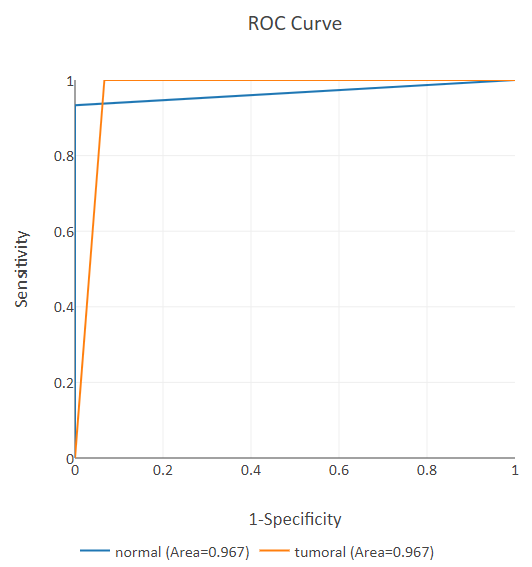
\includegraphics[width=0.4\textwidth]{breast_gse42568_ROC.PNG}}
     \subfloat[Curva A]{
       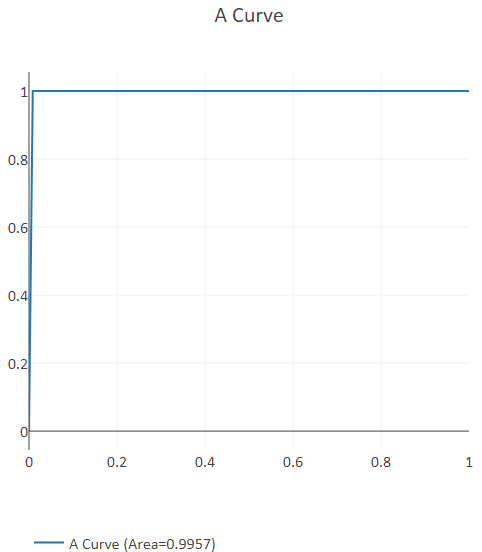
\includegraphics[width=0.4\textwidth]{breast_gse42568_A_CURVE.PNG}}
    \caption{Curvas obtenidas para el fichero breast\_gse42568.csv.}
    \label{fig:13}
\end{figure}

\bigbreak

\lipsum[1]

\clearpage


%%%%%%%%%%%%%%%%%%%%%%%%%%%%%%%%%%%%%%%%%%%%%%%%%%%%%%% RESULTADO

\subsubsection{Fichero gastric\_gse79973.csv}

\begin{table}[htp]
    \small
    \centering
    \begin{tabularx}{\columnwidth}{Y Y}
        ACC       & AUAC    \\\hline
        $0.900$   & $0.921$ \\\hline
    \end{tabularx}
    \caption{Resultados globales para el fichero gastric\_gse79973.csv.}
    \label{tab:18}
\end{table}

\begin{table}[htp]
    \small
    \centering
    \begin{tabularx}{\columnwidth}{l Y Y}
                &  Adenocarcinoma       & Normal        \\\hline
        TPR     &  $0.900$              & $0.900$       \\\hline
        TNR     &  $0.900$              & $0.900$       \\\hline
        PPV     &  $0.900$              & $0.900$       \\\hline
        NPV     &  $0.900$              & $0.900$       \\\hline
        LR+     &  $9.000$              & $9.000$       \\\hline
        LR-     &  $0.111$              & $0.111$       \\\hline
        DOR     &  $81.000$             & $81.000$      \\\hline
        YI      &  $0.800$              & $0.800$       \\\hline
        MCC     &  $0.800$              & $0.800$       \\\hline
        DP      &  $1.052$              & $1.052$       \\\hline
        $F_{1}$ &  $0.900$              & $0.900$       \\\hline
        MK      &  $0.800$              & $0.800$       \\\hline
        BCR     &  $0.900$              & $0.900$       \\\hline
        GM      &  $0.900$              & $0.900$       \\\hline
        OP      &  $0.900$              & $0.900$       \\\hline
        Jaccard &  $0.818$              & $0.818$       \\\hline
    \end{tabularx}
    \caption{Resultados agrupados por clase para el fichero gastric\_gse79973.csv.}
    \label{tab:19}
\end{table}

\bigbreak

\begin{figure}[htp]
    \centering
     \subfloat[Curva ROC]{
       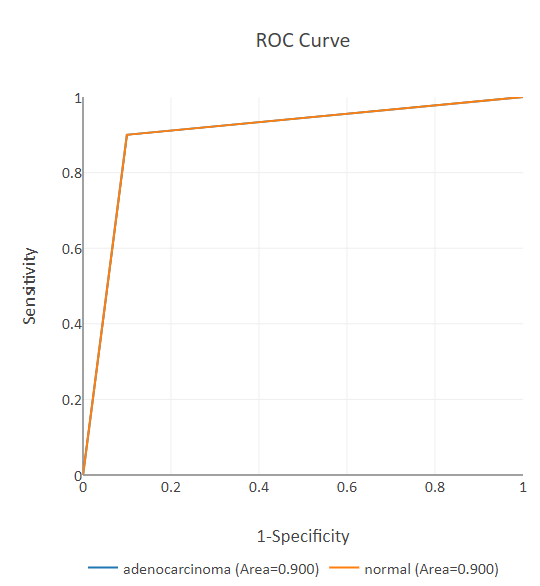
\includegraphics[width=0.4\textwidth]{gastric_gse79973_ROC.PNG}}
     \subfloat[Curva A]{
       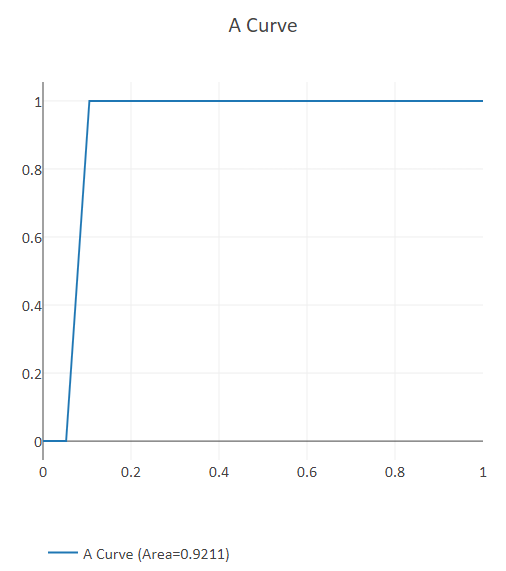
\includegraphics[width=0.4\textwidth]{gastric_gse79973_A_CURVE.PNG}}
    \caption{Curvas obtenidas para el fichero gastric\_gse79973.csv.}
    \label{fig:14}
\end{figure}


La predicción que se realiza a partir de este fichero de datos ofrece unos indicadores de calidad simétricos para ambas clases. La exactitud es de $0.900$ puntos, mientras que el área bajo la curva-A es de $0.921$, esto supone un aumento leve del área bajo la curva en $0.21$ puntos. La sensibilidad, la especificidad, la precisión y la precisión inversa ofrecen el mismo resultado $0.900$, esto indica que los registros de ambas clases, así como, la predicción que se realiza sobre las diferente clases tienen una tasa de acierto del 90\%. EL índice de verosimilitud positiva indica un aumento del 40\% en la probabilidad de que la predicción sea correcta. El índice de verosimilitud negativa indica una disminución del 45\% en la probabilidad de que la predicción se haga de forma incorrecta. El valor de $0.8$ en el indice YI establece una buena capacidad de predicción a partir de la sensibilidad y la especificidad. El coeficiente de correlación de Matthews según la Tabla \ref{tab:3} indica un fuerte grado de correlación entre la clase y la predicción. El DP establece que el modelo presenta una capacidad discriminatoria limitada.

La representación gráfica de la curva ROC ofrece una visión en la que 

\clearpage

%%%%%%%%%%%%%%%%%%%%%%%%%%%%%%%%%%%%%%%%%%%%%%%%%%%%%%% RESULTADO

\subsubsection{Fichero leukemia\_gse14317.csv}

\begin{table}[htp]
    \small
    \centering
    \begin{tabularx}{\columnwidth}{Y Y}
        ACC       & AUAC    \\\hline
        $0.920$   & $0.938$ \\\hline
    \end{tabularx}
    \caption{Resultados globales para el fichero leukemia\_gse14317.csv.}
    \label{tab:20}
\end{table}

\begin{table}[htp]
    \small
    \centering
    \begin{tabularx}{\columnwidth}{l Y Y}
                &  Atl                  & Normal        \\\hline
        TPR     &  $1.000$              & $0.714$       \\\hline
        TNR     &  $0.714$              & $1.000$       \\\hline
        PPV     &  $0.900$              & $1.000$       \\\hline
        NPV     &  $1.000$              & $0.900$       \\\hline
        LR+     &  $3.500$              & -             \\\hline
        LR-     &  $0.000$              & $0.286$       \\\hline
        DOR     &  -                    & -             \\\hline
        YI      &  $0.714$              & $0.714$       \\\hline
        MCC     &  $0.802$              & $0.802$       \\\hline
        DP      &  -                    & -             \\\hline
        $F_{1}$ &  $0.947$              & $0.833$       \\\hline
        MK      &  $0.900$              & $0.900$       \\\hline
        BCR     &  $0.857$              & $0.857$       \\\hline
        GM      &  $0.845$              & $0.845$       \\\hline
        OP      &  $0.753$              & $0.753$       \\\hline
        Jaccard &  $0.900$              & $0.714$       \\\hline
    \end{tabularx}
    \caption{Resultados agrupados por clase para el fichero leukemia\_gse14317.csv.}
    \label{tab:21}
\end{table}

\bigbreak

\begin{figure}[htp]
    \centering
     \subfloat[Curva ROC]{
       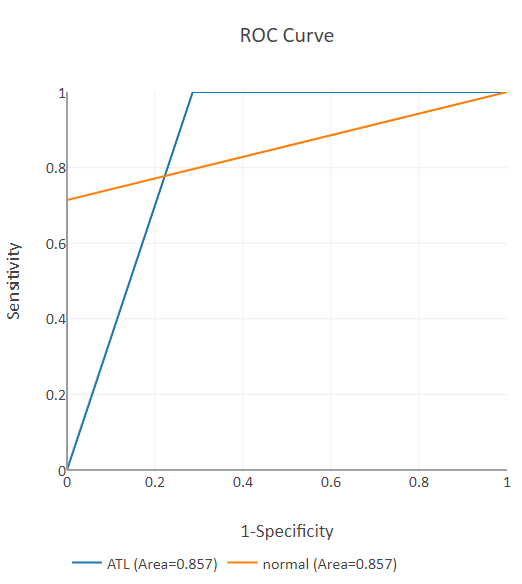
\includegraphics[width=0.4\textwidth]{leukemia_gse14317_ROC.PNG}}
     \subfloat[Curva A]{
       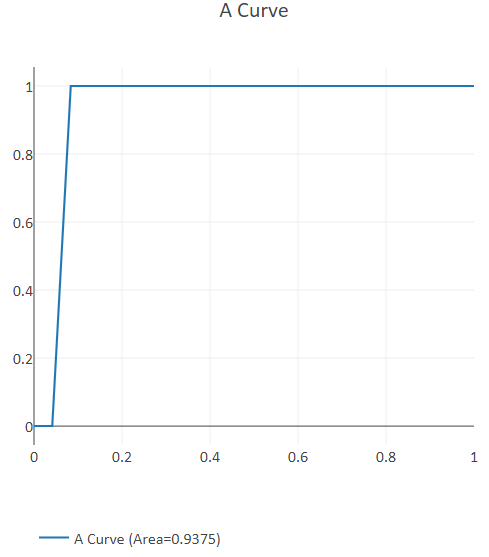
\includegraphics[width=0.4\textwidth]{leukemia_gse14317_A_CURVE.PNG}}
    \caption{Curvas obtenidas para el fichero leukemia\_gse14317.csv.}
    \label{fig:15}
\end{figure}



La exactitud presenta una tasa de aciertos notablemente buena, de cada 100 registros 92 se predicen de forma correcta. El área bajo la curva-A obtiene un valor muy similar al que ha obtenido la exactitud, la diferencia entre ambos métodos supone un aumento en área bajo la curva-A de $0.18$ puntos sobre la exactitud. La sensibilidad y la especificidad representan buenos indicadores, todos los registros de clase Atl se predicen correctamente, los registros de clase Normal tienen un $71.4$\% de probabilidad de acierto. La precisión y la precisión inversa establecen un $90$\% de probabilidad de acierto cuando se predice un registro Atl, por otro la predicción es siempre correcta cuando se predice Normal un registro. El índice de verosimilitud positiva indica un aumento de entorno al 20\% en la probabilidad que tiene un registro que se predice Atl de ser Atl, la clase Normal no presenta índice de verosimilitud positiva debido a que todos los registros que se precicen Normales son efectivamente de clase Normal. El índice de verosimilitud negativa indica que para registros que se predicen de clase Atl hay una reducción del 30\% en la probabilidad de que sea Normal, por otro lado el modelo siempre acierta cuando predice un registro de clase Normal.

\bigbreak

El índice YI presenta un resultado que indica una tasa de aciertos notablemante positiva. El coeficiente de correlación de Matthews de $0.802$ establece una fuerte correlación entre clase y predicción. La medida-F de $0.947$ y $0.833$ implica una que el modelo tiene alta tasa de sensibilidad sobre precisión. El BCR y la GM indican una alta tasa de acierto en la predicción en relación con la sensibilidad y la especificidad del modelo. La precisión de optimización ofrece un resultado en el que se esta penalizando la diferencia entre sensibilidad y especificidad, en valor de $0.714$ en sensibilidad y especificidad implica una reducción leve de la exactitud, sin embargo, a pesar de la penalización sigue ofreciendo un buen nivel de exactitud. El índice de Jaccard establece un nivel de similitud notable entre clase y predicción.

\bigbreak

La representación gráfica que ofrece la curva ROC indican que el modelo ofrece una buena tasa de acierto sobre error en la predicción de ambas clases. La interpretación gráfica de la curva-A establece que la calidad del modelo predictivo es muy positiva.


\clearpage

